% !TeX program = pdflatex
% Parte IV de la serie godsil-gutman-lean.
% Cuando los caminos se vuelven espectro — demostracion verificada por maquina del
% teorema del momento de Godsil p_k = treeLikeWalkCount, en Lean 4.
% Compilar: pdflatex moment-theorem-lean-es.tex  (dos veces, por las referencias)

\documentclass[11pt]{article}
\usepackage[T1]{fontenc}
\usepackage[spanish]{babel}
\usepackage{lmodern}
\usepackage{amsmath,amssymb,amsthm,booktabs,graphicx,hyperref}
\usepackage{xurl}
\usepackage[table]{xcolor}
\definecolor{ggteal}{HTML}{1B6F8C}
\definecolor{ggband}{HTML}{DCE7EB}
\definecolor{ggamber}{HTML}{E08A1E}
\usepackage[margin=1in]{geometry}
\usepackage{microtype}
\usepackage[most]{tcolorbox}
\usepackage{tikz}
\usetikzlibrary{arrows.meta,positioning,fit,backgrounds}
\setlength{\emergencystretch}{2em}
\newtheorem{theorem}{Teorema}
\newtheorem{lemma}{Lema}
\newtheorem{definition}{Definici\'on}
\newcommand{\lean}[1]{\texttt{#1}}
\newcommand{\Z}{\mathbb{Z}}
\newcommand{\R}{\mathbb{R}}
\newcommand{\C}{\mathbb{C}}
\newcommand{\N}{\mathbb{N}}
\DeclareMathOperator{\tr}{tr}
\DeclareMathOperator{\reflect}{reflect}
\DeclareMathOperator{\rev}{rev}
\DeclareMathOperator{\charpolyRev}{charpolyRev}
\providecommand{\llbracket}{[\![}
\providecommand{\rrbracket}{]\!]}
\hypersetup{colorlinks=true,linkcolor=ggteal,citecolor=ggteal,urlcolor=ggteal}
\newtcbox{\keybox}{on line,boxrule=0.9pt,colframe=ggteal,colback=ggband!40,
  arc=3pt,left=8pt,right=8pt,top=5pt,bottom=5pt}
\newcommand{\keyeq}[1]{\begin{center}\keybox{$\displaystyle #1$}\end{center}}
\newtcolorbox{classicalbox}[1][]{colframe=ggteal,colback=ggband!22,boxrule=0.9pt,arc=3pt,
  fonttitle=\bfseries,coltitle=white,colbacktitle=ggteal,title={#1},left=8pt,right=8pt,top=4pt,bottom=4pt}

\title{\bf Cuando los caminos se vuelven espectro\\[4pt]
  \large\normalfont Una demostraci\'on verificada por m\'aquina del teorema del momento de Godsil
  $p_k=\mathrm{treeLikeWalkCount}$, en Lean~4}
\author{Carles Mar\'in\thanks{Formalizado con asistencia de IA (Claude, Anthropic); la matem\'atica y
todas las afirmaciones son responsabilidad del autor. La metodolog\'ia se discute en la
Secci\'on~\ref{sec:methodology}.}\\[3pt]
  \normalsize Investigador independiente\\
  \normalsize \texttt{karlesmarin@gmail.com}}
\date{Junio de 2026}

\begin{document}
\maketitle

\begin{abstract}
Esta es la cuarta pieza de una serie que construye, en Lean~4 / Mathlib, los dos lados de la f\'ormula
de la traza de emparejamientos/Ihara. En \emph{Caminos que olvidan los ciclos}~\cite{PartIII} demostr\'e
la mitad \emph{combinatoria} del teorema del momento de Godsil: los caminos cerrados \emph{tipo
\'arbol} de un grafo $G$ con base en $v$ est\'an en biyecci\'on, que preserva la longitud, con los
caminos cerrados del \'arbol de caminos $T(G,v)$ de Godsil con base en su ra\'iz, de modo que el conteo
de caminos tipo \'arbol es una suma de potencias de matrices de adyacencia,
$\mathrm{treeLikeWalkCount}(G,k)=\sum_v\bigl[A(T(G,v))^k\bigr]_{\mathrm{ra\acute{\imath}z}}$. Aquel
art\'iculo fue expl\'icito sobre su frontera: la mitad \emph{espectral}---convertir esas potencias de
matrices en las sumas de potencias $p_k=\sum_i\theta_i^k$ de las ra\'ices del polinomio de
emparejamientos $\mu(G)$---qued\'o \emph{mapeada, no construida}. Aqu\'i la construyo, y cierro el
teorema:
\[
  p_k(G)\;=\;\sum_i\theta_i^{\,k}\;=\;\mathrm{treeLikeWalkCount}(G,k),
  \qquad\text{verificado por m\'aquina, \lean{sorry}-libre.}
\]
La demostraci\'on es una sola identidad de series formales. En el lado de la traza, el resolvente
ra\'iz--ra\'iz de cada \'arbol de caminos $\sum_k[A(T)^k]_{\mathrm{ra\acute{\imath}z}}X^k$ es, por un
colapso de determinante a un menor principal, el cociente de dos polinomios caracter\'isticos
invertidos; la identidad de divisibilidad de la Parte~II $\mu(G)\mu(T-\mathrm{ra\acute{\imath}z})=\mu(G-v)\mu(T)$
lo reescribe como cociente de polinomios de \emph{emparejamientos} invertidos; sumando sobre $v$ y
aplicando la ley de borrado de v\'ertices $\sum_v\mu(G-v)=X\mu'(G)$ se obtiene
$\mathrm{mk}(\mathrm{treeLikeWalkCount})\cdot\overline{\mu}=\overline{X\mu'}$. En el lado de los
emparejamientos, la funci\'on generatriz de las sumas de potencias de las ra\'ices es igual, tras una
cancelaci\'on de serie geom\'etrica por el producto de factores invertidos, al \emph{mismo} objeto
$\overline{X\mu'}$. Ambos coinciden; cancelar la unidad $\overline{\mu}$ y leer el coeficiente de
$X^k$ es el teorema. Dejo constancia de una sorpresa: la conclusi\'on no necesita \emph{ninguna}
identidad de Newton univariada---la ruta que predijo la entrega anterior---sino solo un manejo, a grado
fijo, de reflexiones de polinomios invertidos. El resultado depende solo de los tres axiomas
est\'andar; no conozco una formalizaci\'on previa del teorema del momento de Godsil en ning\'un
asistente de demostraci\'on. Con esto y el compa\~nero \emph{Bass}, ambos lados de la f\'ormula de la
traza finita quedan, \lean{sorry}-libres, en una sola biblioteca.
\end{abstract}

\noindent\emph{Mapa del lector.} Si lee una sola cosa, lea el Teorema~\ref{thm:moment} y la forma de
su demostraci\'on: \emph{ambas} funciones generatrices, la que cuenta caminos y la de las sumas de
potencias de autovalores, son forzadas a igualar uno y el mismo polinomio invertido
$\overline{X\mu'(G)}$ (Figura~\ref{fig:weld}). Todo lo dem\'as es la versi\'on cuidadosa de esa frase:
una identidad por v\'ertice que convierte el lado de la traza en polinomios de emparejamientos
invertidos (Secci\'on~\ref{sec:trace}), una cancelaci\'on de serie geom\'etrica que convierte el lado
de los emparejamientos en lo mismo (Secci\'on~\ref{sec:match}), y una extracci\'on de coeficiente una
vez cancelada una unidad (Secci\'on~\ref{sec:weld}). La sorpresa honesta---sin Newton---es la
Secci\'on~\ref{sec:boundary}; los l\'imites y la metodolog\'ia, la Secci\'on~\ref{sec:methodology};
las pr\'oximas preguntas, la Secci\'on~\ref{sec:questions}.

% ---------------------------------------------------------------
\section{Introducci\'on: un conteo, y el espectro que esconde}
\label{sec:intro}

\emph{El polinomio de emparejamientos de un grafo no es el polinomio caracter\'istico de su matriz de
adyacencia---\,?`d\'onde viven entonces las sumas de potencias de sus ra\'ices, y por qu\'e son un
conteo de caminos?} La entrega anterior respondi\'o la primera cl\'ausula con un \'arbol y dej\'o la segunda
como pagar\'e; este art\'iculo lo salda. La ruta tiene una historia larga---cuatro siglos---y una
peque\~na sorpresa esperando en su \'ultimo paso (Secci\'on~\ref{sec:boundary}).

\paragraph{Un hilo, en cinco cuentas.} En 1629 Albert Girard escribi\'o lo que Newton
sistematizar\'ia una generaci\'on despu\'es: las sumas de potencias $p_k=\sum_i\theta_i^k$ de las
ra\'ices de un polinomio quedan fijadas por sus coeficientes y, rec\'iprocamente, por una recursi\'on
que hoy lleva el nombre de Newton~\cite{Girard,Macdonald}. Esa recursi\'on es el puente can\'onico
entre las ra\'ices de un polinomio y sus datos, y ser\'a la cuenta que este art\'iculo, justo al final,
declina usar. En 1972 Heilmann y Lieb produjeron un polinomio que parec\'ia no tener derecho alguno a
ra\'ices reales---el polinomio de emparejamientos de un grafo, nacido en la mec\'anica estad\'istica de
los sistemas mon\'omero--d\'imero---y demostraron sus ra\'ices reales de todos
modos~\cite{HeilmannLieb}, aunque no es el polinomio caracter\'istico de la matriz de adyacencia del
grafo salvo que sea un bosque. En 1981 Godsil resolvi\'o la paradoja con un solo dispositivo, el
\emph{\'arbol de caminos}, y extrajo de \'el \emph{dos} conclusiones: que el polinomio de
emparejamientos tiene ra\'ices reales (divide al de un bosque, y los bosques tienen espectros
sim\'etricos), y que las sumas de potencias de sus ra\'ices \emph{cuentan
caminos}~\cite{Godsil1981a,GodsilBook}. La cuarta cuenta es el \emph{cubrimiento universal}: el
\'arbol de caminos es su truncaci\'on finita, el borde espectral del cubrimiento $2\sqrt{\Delta-1}$ es
la cota de Godsil sobre las ra\'ices de emparejamiento y el umbral de
Ramanujan~\cite{AngelFriedmanHoory,McKay,MSS}, y el conteo de caminos es una sombra finita de una
f\'ormula de la traza sobre el cubrimiento. La quinta cuenta es esta serie: la Parte~II llev\'o la
primera conclusi\'on de Godsil a Lean~\cite{PartII}, la Parte~III llev\'o la mitad combinatoria de la
segunda~\cite{PartIII}, y este art\'iculo lleva el resto---y, al ensartar la \'ultima cuenta, vuelve
inesperadamente a la primera (Secci\'on~\ref{sec:boundary}).

\paragraph{El polinomio fuera del espectro de adyacencia.} Un grafo finito $G$ de $n$ v\'ertices porta
un polinomio de emparejamientos $\mu(G,x)=\sum_k(-1)^k m_k(G)x^{n-2k}$, con $m_k(G)$ el n\'umero de
emparejamientos de $k$ aristas~\cite{Farrell1979,LovaszPlummer}. Heilmann y Lieb demostraron que sus
ra\'ices $\theta_1,\dots,\theta_n$ son reales~\cite{HeilmannLieb}; pero $\mu(G)$ es igual al polinomio
caracter\'istico de la matriz de adyacencia $A(G)$ solo cuando $G$ es un bosque.\footnote{Todo
polinomio m\'onico es, trivialmente, el polinomio caracter\'istico de su matriz compa\~nera, y---al
tener ra\'ices reales---de $\mathrm{diag}(\theta_1,\dots,\theta_n)$. Lo relevante es que $\mu(G)$ no es
el polinomio caracter\'istico de la matriz construida \emph{can\'onicamente a partir del grafo}, su
matriz de adyacencia, salvo que $G$ sea un bosque. Agradecemos a Scott Hotton el haber suscitado esta
aclaraci\'on.} Sus sumas de potencias $p_k(G)=\sum_i\theta_i^k$ son, por tanto, los momentos de un
espectro \emph{fantasma}: n\'umeros reales que se comportan como autovalores, pero no los de la matriz
de adyacencia del propio grafo. El teorema del momento de Godsil
dice de d\'onde salen: \emph{cuentan caminos}.

\paragraph{Un \'arbol, dos teoremas.} El dispositivo de Godsil~\cite{Godsil1981a,Godsil1981b,GodsilBook}
es el \'arbol de caminos $T(G,v)$, cuyos v\'ertices son los caminos simples de $G$ desde $v$ y cuyas
aristas son extensiones de una sola arista. Es un bosque---una truncaci\'on finita del cubrimiento
universal desplegado desde $v$---y la Parte~II de esta serie~\cite{PartII} lo us\'o para verificar por
m\'aquina Heilmann--Lieb: $\mu(G)$ divide a $\mu(T(G,v))$, y el polinomio de emparejamientos de un
bosque \emph{es} su polinomio caracter\'istico de adyacencia, luego de ra\'ices reales. La
Parte~III~\cite{PartIII} ense\~n\'o al mismo \'arbol a contar: un camino cerrado de $G$ es \emph{tipo
\'arbol} cuando en cada paso avanza a un v\'ertice nuevo o retrocede a su padre, sin cerrar nunca a
sabiendas un ciclo, y los caminos cerrados tipo \'arbol de $G$ en $v$ son exactamente los caminos
cerrados de $T(G,v)$ en su ra\'iz, proyectados hacia abajo registrando el extremo actual. La
consecuencia,
\keyeq{\mathrm{treeLikeWalkCount}(G,k)\;=\;\sum_{v}\bigl[A(T(G,v))^{k}\bigr]_{\mathrm{ra\acute{\imath}z}},}
es el resultado central de la Parte~III (\lean{treeLikeWalkCount\_eq\_sum\_pathTree\_adjMatrix\_pow}).
Pero la Parte~III marc\'o con cuidado su frontera: la igualdad de este conteo con los momentos
$p_k$---la mitad \emph{espectral}---qued\'o mapeada en su secci\'on de cierre, no formalizada.
Este art\'iculo la construye. El enunciado que se construye es el de Godsil, en su forma cl\'asica:

\begin{classicalbox}[Teorema del momento de Godsil (1981, forma cl\'asica)~\cite{Godsil1981a}]
Sea $G$ un grafo finito de $n$ v\'ertices, con polinomio de emparejamientos $\mu(G,x)$ de ra\'ices
reales $\theta_1,\dots,\theta_n$. Para todo $k\ge0$,
\[
  p_k(G)\;=\;\sum_{i=1}^{n}\theta_i^{\,k}\;=\;\#\{\text{caminos cerrados tipo \'arbol de longitud }k\text{ en }G\}.
\]
\end{classicalbox}
\noindent El Teorema~\ref{thm:moment} de m\'as abajo es la forma verificada por m\'aquina de este
enunciado.

\paragraph{Qu\'e significa ``construirla''.} Las dos mitades son dos funciones generatrices:
$\mathrm{mk}(k\mapsto\mathrm{treeLikeWalkCount}(G,k))$ en el lado de la traza y $\mathrm{mk}(k\mapsto
p_k(G))$ en el de los emparejamientos, ambas elementos de un anillo de series formales. El teorema es
que son iguales; por debajo del cuello (\emph{girth}) sus coeficientes ya coinciden (todo camino corto
es tipo \'arbol), pero el enunciado completo es una sola identidad en $\R\llbracket X\rrbracket$
empujada a $\C\llbracket X\rrbracket$ para dar sitio a las ra\'ices complejas. La estrategia: mostrar
que cada lado, multiplicado por el polinomio de emparejamientos \emph{invertido} $\overline{\mu(G)}$,
iguala uno y el mismo polinomio invertido $\overline{X\mu'(G)}$; como $\overline{\mu(G)}$ es una unidad
(su t\'ermino constante es el coeficiente principal $1$ del m\'onico $\mu$), las dos generatrices
coinciden, y el coeficiente de $X^k$ es el teorema.

\paragraph{Qu\'e es nuevo, y qu\'e no.} La contribuci\'on se separa con nitidez. La \emph{matem\'atica}
es de Godsil, de hace cuatro d\'ecadas; nada del enunciado cl\'asico de arriba es nuevo. Lo nuevo es,
primero, su \emph{certificaci\'on completa por m\'aquina}---la primera que conozco en cualquier
asistente de demostraci\'on---y, segundo, un pu\~nado de \emph{lemas generales} que la certificaci\'on
oblig\'o a construir y que no exist\'ian en Mathlib (la Tabla~\ref{tab:deps} traza las entradas).

\paragraph{Por qu\'e no fue rutinario formalizarlo.} Un polinomio de emparejamientos no es el polinomio
caracter\'istico de la matriz de adyacencia del grafo, as\'i que ninguna de las herramientas matriciales se le aplica
directamente; la demostraci\'on debe pasar por el \'arbol de caminos de Godsil y volver, y cada cruce
es una coerci\'on entre un polinomio, su \emph{invertido} y una serie formal---contabilidad que Mathlib
no empaqueta. Hubo que llenar tres huecos concretos. (i)~La identidad de cofactores de Mathlib
$\mathrm{adj}(M)_{ii}=\det(M\!\restriction_{j\neq i})$ exist\'ia solo para el tipo de \'indice
\lean{Fin\,n}; los \'indices del \'arbol de caminos son un tipo finito arbitrario, as\'i que hizo falta
una demostraci\'on sin base, triangular en bloques. (ii)~No hab\'ia lema de que una suma de polinomios
del mismo grado se invierta t\'ermino a t\'ermino ($\reflect_N$ es aditiva, $\rev$ no), el hecho que
permite sumar las piezas por v\'ertice. (iii)~El invertido de un producto descompuesto,
$\rev\prod(X-\theta)=\prod(1-\theta X)$, y la cancelaci\'on de serie geom\'etrica que sustituye a la
recursi\'on de Newton, faltaban igualmente. Ninguno es profundo; cada uno es general, y todos se guardan
libres de grafos para su env\'io aguas arriba. El resultado, \lean{matchingPowerSum\_eq\_treeLikeWalkCount},
depende solo de \lean{propext}, \lean{Classical.choice} y \lean{Quot.sound}; no hay \lean{sorry}, como
confirmar\'a \lean{\#print axioms}.

\begin{table}[h]
\centering\small
\caption{En qu\'e se apoya este art\'iculo. Las dos partes precedentes aportan las ra\'ices reales y la
biyecci\'on combinatoria; este art\'iculo aporta la conclusi\'on espectral que las une en el teorema
del momento.}
\label{tab:deps}
\rowcolors{2}{ggband!30}{white}
\begin{tabular}{@{}lll@{}}
\toprule
\rowcolor{ggteal}
{\color{white}\textbf{Ingrediente}} & {\color{white}\textbf{Enunciado}} & {\color{white}\textbf{Fuente}}\\
\midrule
Heilmann--Lieb / ra\'ices reales & $\mu(G)\mid\mu(T(G,v))$, bosques de ra\'ices reales & Parte~II~\cite{PartII}\\
Biyecci\'on de caminos tipo \'arbol & $\mathrm{tlwc}(G,k)=\sum_v[A(T(G,v))^k]_{\rm ra\acute{\imath}z}$ & Parte~III~\cite{PartIII}\\
Identidad de divisibilidad & $\mu(G)\mu(T{-}r)=\mu(G{-}v)\mu(T)$ & Parte~II~\cite{PartII}\\
\textbf{Conclusi\'on espectral} & \textbf{$p_k=\mathrm{tlwc}(G,k)$ (el teorema del momento)} & \textbf{este art\'iculo}\\
\bottomrule
\end{tabular}
\end{table}

\begin{figure}[t]
\centering
\begin{tikzpicture}[
  font=\scriptsize,
  node distance=4.5mm,
  ext/.style={draw=ggteal!55,dashed,rounded corners=2pt,fill=white,inner sep=3.5pt,align=center},
  st/.style={draw=ggteal,rounded corners=2pt,fill=ggband!40,inner sep=3.5pt,align=center},
  goal/.style={draw=ggamber,line width=1pt,rounded corners=2pt,fill=ggamber!14,inner sep=4.5pt,align=center},
  fl/.style={-{Stealth[length=1.7mm]},ggteal!85,semithick}]
\node[ext] (p2) at (0,1.5) {\textbf{Parte~II}\\ \lean{godsil\_identity}\\ $\mu(G)\mu(T{-}r){=}\mu(G{-}v)\mu(T)$};
\node[ext] (p3) at (0,-1.5) {\textbf{Parte~III}\\ \lean{...adjMatrix\_pow}\\ $\mathrm{tlwc}=\sum_v[A(T)^k]_{\rm ra\acute{\imath}z}$};
\node[st] (s3) at (4.1,1.9) {Stone 3 $+$ M1\\ resolvente $=$\\ cociente de menores};
\node[st] (m3) at (4.1,0.4) {M3 por v\'ertice\\ $(\,\sum_k\cdots)\overline{\mu(G)}{=}\overline{\mu(G{-}v)}$};
\node[st] (m4) at (8.1,1.2) {M4 lado traza\\ $W(G)\overline{\mu(G)}{=}\overline{X\mu'}$};
\node[st] (s4) at (4.1,-1.2) {Stone 4 $+(\star)$\\ $\sum_\theta\mathrm{geom}\cdot\!\prod(1{-}\theta X)$};
\node[st] (m5) at (8.1,-1.2) {M5 lado empar.\\ $M(G)\overline{\mu_\C}{=}\overline{X\mu_\C'}$};
\node[goal] (thm) at (12.0,0) {\textbf{M6 t.\ momento}\\ \lean{matchingPowerSum}\\ \lean{\_eq\_treeLikeWalkCount}};
\draw[fl] (p2) -- (s3); \draw[fl] (p2) -- (m3);
\draw[fl] (p3) -- (m4.west);
\draw[fl] (s3) -- (m3); \draw[fl] (m3) -- (m4);
\draw[fl] (s4) -- (m5);
\draw[fl] (m4) -- (thm); \draw[fl] (m5) -- (thm);
\draw[fl,ggamber] (m4) to[bend left=10] node[above,font=\tiny,text=ggamber]{$\R\to\C$, cancelar $\overline{\mu}$} (thm);
\end{tikzpicture}
\caption{Mapa de dependencias formales. Dos entradas externas (Partes~II y~III, discontinuas)
alimentan una columna de traza y una de emparejamientos; cada una termina en la misma derivada
reflejada $\overline{X\mu'}$ (M4 sobre $\R$, M5 sobre $\C$); el cambio de base $\R\to\C$ y la
cancelaci\'on de la unidad $\overline{\mu}$ cierran el teorema del momento (M6, \'ambar). Cada caja es
un resultado de Lean \lean{sorry}-libre; cf.\ Tabla~\ref{tab:results}.}
\label{fig:roadmap}
\end{figure}

% ---------------------------------------------------------------
\section{Las dos funciones generatrices}
\label{sec:objects}

\emph{\,?`Cu\'ales son los dos objetos, y en qu\'e anillo se encuentran?} Mantenerlos honestamente
aparte importa, porque todo el contenido es que coinciden. El lado de la traza es un conteo de
n\'umeros naturales; el de los emparejamientos vive sobre $\C$, porque las ra\'ices lo hacen.

El lado de la traza es la serie formal cuyo $k$-\'esimo coeficiente es el conteo tipo \'arbol,
\[
  W(G)\;:=\;\mathrm{mk}\bigl(k\mapsto(\mathrm{treeLikeWalkCount}(G,k):\R)\bigr)\ \in\ \R\llbracket X\rrbracket .
\]
Por la forma espectral de la Parte~III es una suma de resolventes ra\'iz--ra\'iz de los \'arboles de
caminos; lo mantendremos sobre $\R$ tanto como podamos y cruzaremos a $\C$ solo al final. El lado de
los emparejamientos es
\[
  M(G)\;:=\;\mathrm{mk}\bigl(k\mapsto p_k(G)\bigr)\ \in\ \C\llbracket X\rrbracket,
  \qquad p_k(G)=\sum_{\theta\in\mathrm{ra\acute{\imath}ces}(\mu_\C)}\theta^{k},
\]
donde $\mu_\C:=\mu(G)$ aplicado a lo largo de $\R\hookrightarrow\C$, de modo que su multiconjunto de
ra\'ices tiene exactamente $n=|V(G)|$ elementos (\lean{matchingPowerSum}, \lean{matchingPowerSum\_genfun}).
La demostraci\'on iguala las im\'agenes de $W(G)$ y $M(G)$ en $\C\llbracket X\rrbracket$.

En todo el texto, $\overline{p}$ denota la coerci\'on del polinomio invertido $\rev(p)=\reflect_{\deg
p}(p)$ a un anillo de series, y $\reflect_N$ es la reflexi\'on a grado $N$, $x^j\mapsto x^{N-j}$. El
\'unico hecho algebraico en que nos apoyamos repetidamente es que $\reflect_N$ es aditiva en $p$ a una
longitud \emph{fija} $N$, aunque $\rev$ (que refleja al grado propio de cada polinomio) no lo sea.

% ---------------------------------------------------------------
\section{El lado de la traza se vuelve un polinomio de emparejamientos invertido}
\label{sec:trace}

\emph{La Parte~III dej\'o el lado de la traza como suma de potencias de matrices de \'arboles.
\,?`C\'omo una suma sobre \'arboles de caminos, cada uno un bosque distinto, se vuelve un enunciado
sobre el propio polinomio de emparejamientos de $G$?} Por tres movimientos: un colapso de determinante
que identifica el numerador del resolvente, la identidad de divisibilidad de la Parte~II que cambia el
\'arbol por el grafo, y una reflexi\'on que suma las piezas. La funci\'on generatriz de caminos de un
grafo es ella misma un objeto cl\'asico~\cite{GodsilMoments}; lo nuevo es el camino verificado por
m\'aquina desde ella hasta el polinomio de emparejamientos.

\paragraph{El resolvente por \'arbol.} Para cualquier matriz $M$ sobre un anillo conmutativo e
\'indice $i$, la diagonal del resolvente genera las potencias diagonales,
\[
  \Bigl(\sum_{k\ge0}[M^k]_{ii}X^k\Bigr)\cdot\overline{\charpolyRev(M)}
  \;=\;\overline{\charpolyRev\bigl(M\!\restriction_{j\neq i}\bigr)},
\]
el caso de una sola entrada de la regla de Cramer, donde $\charpolyRev(M)=\det(1-XM)$ es el polinomio
caracter\'istico invertido (\lean{resolventGenfun\_diag\_mul\_coe\_charpolyRev}). Su demostraci\'on
necesit\'o un lema general ausente de Mathlib: la identidad del menor principal
$\mathrm{adj}(M)_{ii}=\det(M\!\restriction_{j\neq i})$ sobre un tipo de \'indice finito arbitrario, que
demostramos por una reindexaci\'on triangular en bloques $n\simeq\{i\}\sqcup\{j\neq i\}$ en lugar de la
expansi\'on por cofactores solo para \lean{Fin} que Mathlib lleva
(\lean{adjugate\_diag\_eq\_det\_submatrix\_ne}).

\paragraph{De la submatriz a la ra\'iz aislada.} La forma espectral de la Parte~III borra la ra\'iz
como \emph{\'indice} de matriz; la identidad de divisibilidad de la Parte~II habla de borrar sus
\emph{aristas}. Hay que reconciliarlas. Borrar todas las aristas en la ra\'iz $r$ de $T=T(G,v)$ deja
una fila nula, as\'i que $1-X\,A(T_{\widehat r})$ tiene su fila $r$ igual al vector b\'asico $e_r$, y
su determinante colapsa al menor $\{j\neq r\}$---que es exactamente la submatriz que produjo el
resolvente. Luego
\keyeq{\overline{\charpolyRev\bigl(A(T_{\widehat r})\bigr)}\;=\;\overline{\charpolyRev\bigl(A(T)\!\restriction_{j\neq
r}\bigr)},}
el puente entre los dos borrados (\lean{coe\_charpolyRev\_adjMatrix\_deleteIncidenceSet}, apoyado en el
general \lean{det\_eq\_det\_submatrix\_ne\_of\_row\_eq\_single}).

\paragraph{La identidad por v\'ertice.} Ahora entra la Parte~II. Invirtiendo la identidad de
divisibilidad $\mu(G)\,\mu(T_{\widehat r})=\mu(G-v)\,\mu(T)$ sobre el dominio \'integro $\R[X]$ (la
inversi\'on es multiplicativa all\'i, y $\rev\circ\det=\charpolyRev$), el puente del bosque
$\mu(T)=\det(xI-A(T))$ convierte cada polinomio de emparejamientos invertido en un $\charpolyRev$; al cancelar
el factor unidad com\'un $\overline{\charpolyRev(A(T))}$ colapsa toda la historia por \'arbol a un solo
enunciado limpio sobre $G$:
\keyeq{\Bigl(\sum_k[A(T(G,v))^k]_{\mathrm{ra\acute{\imath}z}}X^k\Bigr)\cdot\overline{\mu(G)}\;=\;\overline{\mu(G-v)} }
(\lean{resolventGenfun\_pathTree\_mul\_reverse\_matchingPoly}; aqu\'i $G-v$ es la forma de borrado de
incidencia, que a\'isla $v$). El \'arbol de caminos hizo su trabajo y desapareci\'o: solo quedan
$\mu(G)$ y $\mu(G-v)$.

\paragraph{Sumando sobre $v$.} Sumando la identidad por v\'ertice sobre todos los v\'ertices, el lado
izquierdo se vuelve $W(G)\cdot\overline{\mu(G)}$ (la forma espectral de la Parte~III, con una coerci\'on
$\N\to\R$ que aporta \lean{Matrix.map\_pow}). El derecho es $\sum_v\overline{\mu(G-v)}$, y aqu\'i la
contabilidad de reflexi\'on da su fruto: todo $\mu(G-v)$ tiene el mismo grado $n$, as\'i que las inversiones
comparten longitud y $\sum_v\rev(\mu(G-v))=\reflect_n(\sum_v\mu(G-v))$ (\lean{sum\_reverse\_eq\_reflect\_sum}).
La ley derivada de borrado de v\'ertices $\sum_v\mu(G-v)=X\,\mu'(G)$
(\lean{sum\_matchingPoly\_deleteIncidenceSet}) cierra el movimiento:
\keyeq{W(G)\cdot\overline{\mu(G)}\;=\;\overline{X\,\mu'(G)}.}
Todo el lado de la traza es ahora un polinomio de emparejamientos reflejado
(\lean{mk\_treeLikeWalkCount\_mul\_reverse\_eq}). Usar $\reflect_n$, en vez de $\rev$, para el numerador
es lo que permite no calcular nunca el grado de $X\mu'$.

% ---------------------------------------------------------------
\section{El lado de los emparejamientos se vuelve lo mismo}
\label{sec:match}

\emph{El lado de los emparejamientos no sabe nada de \'arboles; solo sabe de las ra\'ices.
\,?`C\'omo la generatriz de $\sum_i\theta_i^k$ se vuelve el mism\'isimo $\overline{X\mu'}$?} Por una
serie geom\'etrica que cancela un producto, y el hecho cl\'asico de que la derivada de un polinomio es
la suma de sus productos de factores ``dejando uno fuera''.

\paragraph{Sumas de potencias como series geom\'etricas.} La generatriz de las sumas de potencias es,
coeficiente a coeficiente, la suma sobre el multiconjunto de series geom\'etricas por ra\'iz,
\[
  M(G)\;=\;\sum_{\theta}\mathrm{geomSeries}(\theta),\qquad
  \mathrm{geomSeries}(\theta)=\sum_k\theta^kX^k=(1-\theta X)^{-1}
\]
(\lean{powerSum\_genfun}). Multiplicar por el producto de factores invertidos la colapsa, ra\'iz por
ra\'iz: como $\mathrm{geomSeries}(\theta)\,(1-\theta X)=1$ y el producto entero
$\prod_\theta(1-\theta X)$ se factoriza como $(1-\theta X)$ por el producto sin ese factor, se obtiene
\keyeq{\Bigl(\sum_\theta\mathrm{geomSeries}(\theta)\Bigr)\cdot\!\prod_\theta(1-\theta X)\;=\;\sum_\theta\!\prod_{\varphi\neq\theta}(1-\varphi X)}
\emph{sin} derivada y \emph{sin} recursi\'on de Newton---solo la cancelaci\'on de un factor
(\lean{geomSeries\_sum\_mul\_prod}). Como $\mu_\C$ es m\'onico y se descompone sobre $\C$, es igual a
$\prod_\theta(X-\theta)$, y la inversi\'on env\'ia esto a $\prod_\theta(1-\theta X)$
(\lean{reverse\_prod\_X\_sub\_C}); luego el factor izquierdo es $\overline{\mu_\C}$.

\paragraph{La suma ``dejando uno fuera'' es la derivada reflejada.} El lado derecho es el espejo, en
emparejamientos, del numerador del lado de la traza. Cl\'asicamente, para un polinomio descompuesto,
$\mu_\C'=\sum_\theta\prod_{\varphi\neq\theta}(X-\varphi)$ (\lean{derivative\_prod\_X\_sub\_C}, la regla
del producto). Cada producto ``dejando uno fuera'' tiene grado $n-1$, as\'i que
$X\cdot\prod_{\varphi\neq\theta}(X-\varphi)$ tiene grado $n$; reflejando a la longitud fija $n$ y
usando $\rev(Xq)=\rev(q)$ t\'ermino a t\'ermino,
\keyeq{\sum_\theta\prod_{\varphi\neq\theta}(1-\varphi X)\;=\;\reflect_n\!\bigl(X\,\mu_\C'\bigr)}
(\lean{reflect\_X\_mul\_derivative\_eq\_sum\_prod}). Encadenando las dos cajas a trav\'es de la
coerci\'on a series de un producto y de una suma se obtiene el an\'alogo, en emparejamientos, de la
identidad de la traza,
\keyeq{M(G)\cdot\overline{\mu_\C}\;=\;\overline{X\,\mu_\C'}}
(\lean{mk\_powerSum\_mul\_reverse}, especializado a $\mu_\C$ en
\lean{mk\_matchingPowerSum\_mul\_reverse\_eq}). Ambos lados hablan ya del mismo polinomio reflejado.

% ---------------------------------------------------------------
\section{La soldadura}
\label{sec:weld}

\emph{Dos identidades, una sobre $\R$ y otra sobre $\C$, ambas terminando en $\overline{X\mu'}$.
\,?`Qu\'e queda sino juntarlas?} Un cambio de base y una cancelaci\'on.

La identidad de la traza vive sobre $\R$; la de los emparejamientos sobre $\C$. Aplicar a la primera el
homomorfismo de anillos $\R\to\C$ conmuta con todo lo que importa---con $\mathrm{mk}$ (v\'ia
\lean{coeff\_map} y las coerciones de $\N$), con la coerci\'on de polinomio a serie, con $\rev$ (que es
$\reflect$ a un grado preservado por una aplicaci\'on inyectiva), con $\reflect$, y con la derivada
(\lean{reflect\_map}, \lean{derivative\_map}, \lean{natDegree\_map\_eq\_of\_injective}). La imagen de la
identidad de la traza es por tanto
\[
  W_\C(G)\cdot\overline{\mu_\C}\;=\;\overline{X\,\mu_\C'},
  \qquad W_\C(G)=\mathrm{mk}\bigl(k\mapsto(\mathrm{treeLikeWalkCount}(G,k):\C)\bigr),
\]
id\'entica en su lado derecho a la identidad de los emparejamientos
$M(G)\cdot\overline{\mu_\C}=\overline{X\mu_\C'}$. Luego
$W_\C(G)\cdot\overline{\mu_\C}=M(G)\cdot\overline{\mu_\C}$. El polinomio de emparejamientos invertido
$\overline{\mu_\C}$ es una unidad: $\mu_\C$ es m\'onico, as\'i que $\rev(\mu_\C)$ tiene t\'ermino
constante $1$ y es no nulo, y $\C\llbracket X\rrbracket$ es un dominio \'integro. Cancelarlo da
$W_\C(G)=M(G)$, y leer el coeficiente de $X^k$ es el teorema.

\begin{theorem}[Teorema del momento de Godsil, verificado por m\'aquina]
\label{thm:moment}
Para todo grafo finito $G$ sobre el tipo de v\'ertices $V$, y todo $k\in\N$,
\[
  p_k(G)\;=\;\sum_{\theta\in\mathrm{ra\acute{\imath}ces}(\mu_\C)}\theta^{\,k}\;=\;\bigl(\mathrm{treeLikeWalkCount}(G,k):\C\bigr).
\]
En Lean: \lean{matchingPowerSum\_eq\_treeLikeWalkCount}. La demostraci\'on es \lean{sorry}-libre y
depende solo de \lean{propext}, \lean{Classical.choice}, \lean{Quot.sound}.
\end{theorem}

\begin{figure}[t]
\centering
\begin{tikzpicture}[
  font=\small,
  box/.style={draw=ggteal,rounded corners=2pt,fill=ggband!35,inner sep=5pt,align=center},
  meet/.style={draw=ggamber,line width=1pt,rounded corners=2pt,fill=ggamber!12,inner sep=6pt,align=center},
  ar/.style={-{Stealth[length=2mm]},ggteal,thick}]
\node[box] (w) at (0,2.1) {$W(G)=\mathrm{mk}\,(\mathrm{treeLikeWalkCount})$\\[2pt]\footnotesize lado de la traza, sobre $\R$};
\node[box] (m) at (0,-2.1) {$M(G)=\mathrm{mk}\,(p_k)$\\[2pt]\footnotesize lado de emparejamientos, sobre $\C$};
\node[box] (wt) at (6.2,2.1) {$W(G)\cdot\overline{\mu(G)}$\\[2pt]\footnotesize Stone 1\,$+$\,resolvente\\\footnotesize $+$ divisibilidad Parte~II};
\node[box] (mt) at (6.2,-2.1) {$M(G)\cdot\overline{\mu_\C}$\\[2pt]\footnotesize serie geom\'etrica\\\footnotesize $+$ descomposici\'on};
\node[meet] (mid) at (11.3,0) {$\overline{X\,\mu'(G)}$\\[2pt]\footnotesize la derivada\\\footnotesize reflejada com\'un};
\draw[ar] (w) -- (wt);
\draw[ar] (m) -- (mt);
\draw[ar] (wt) -- node[above,sloped,font=\scriptsize]{$\sum_v$, borrado de v\'ertices} (mid);
\draw[ar] (mt) -- node[below,sloped,font=\scriptsize]{$\reflect_n$, regla del producto} (mid);
\draw[{Stealth[length=2mm]}-{Stealth[length=2mm]},ggamber,thick,dashed]
  (w) to[bend left=18] node[above,font=\scriptsize,text=ggamber]{cancelar $\overline{\mu}$ (unidad) $\Rightarrow$ iguales} (m);
\end{tikzpicture}
\caption{La soldadura. Ambas generatrices, multiplicadas por el polinomio de emparejamientos
invertido, son forzadas a igualar la misma derivada reflejada $\overline{X\mu'(G)}$ (sobre $\R$
arriba, sobre $\C$ abajo, unidas por el cambio de base $\R\to\C$). Cancelar la unidad $\overline{\mu}$
identifica las dos series; el coeficiente de $X^k$ es el teorema del momento.}
\label{fig:weld}
\end{figure}

% ---------------------------------------------------------------
\section{Verificaci\'on num\'erica}
\label{sec:numeric}

\emph{Una demostraci\'on formal certifica la implicaci\'on; \,?`qu\'e certifica que el enunciado
formalizado es el que se pretend\'ia?} Cada identidad de este art\'iculo se de-arriesg\'o
num\'ericamente antes de todo esfuerzo formal, contra aritm\'etica exacta, y las mismas comprobaciones
fijan los dos lados del teorema, uno junto al otro. Vale la pena ver el teorema aterrizar entero sobre
un grafo peque\~no.

\paragraph{Un ejemplo trabajado: el pent\'agono $C_5$.} Tomemos el $5$-ciclo. Sus emparejamientos son
el vac\'io, las cinco aristas sueltas, y los cinco pares de aristas no adyacentes, as\'i que
$m_0=1,\,m_1=5,\,m_2=5$ y
\[
  \mu(C_5,x)\;=\;x^5-5x^3+5x\;=\;x\Bigl(x^2-\tfrac{5+\sqrt5}{2}\Bigr)\Bigl(x^2-\tfrac{5-\sqrt5}{2}\Bigr),
\]
con ra\'ices $\theta\in\bigl\{0,\ \pm\sqrt{(5+\sqrt5)/2},\ \pm\sqrt{(5-\sqrt5)/2}\bigr\}$. El lado de
los \emph{emparejamientos} lee las sumas de potencias de estas ra\'ices:
\[
  p_2=\sum_i\theta_i^2=\tfrac{5+\sqrt5}{2}\cdot2+\tfrac{5-\sqrt5}{2}\cdot2=10,
  \qquad
  p_4=\sum_i\theta_i^4=\Bigl(\tfrac{5+\sqrt5}{2}\Bigr)^{\!2}\!\cdot2+\Bigl(\tfrac{5-\sqrt5}{2}\Bigr)^{\!2}\!\cdot2=30.
\]
El lado \emph{tipo \'arbol} cuenta caminos. Para $k=2$, un camino cerrado tipo \'arbol en un v\'ertice
va a un vecino y vuelve; cada uno de los $5$ v\'ertices tiene $2$ vecinos, lo que da $2\cdot5=10=p_2$.
Para $k=4$, el cuello de $C_5$ es $5$, as\'i que \emph{todo} camino cerrado de longitud $4$ es tipo
\'arbol (ninguno puede a\'un encerrar el pent\'agono), y el conteo es
$\tr(A^4)=2^4+2\bigl(\tfrac{\sqrt5-1}{2}\bigr)^4+2\bigl(\tfrac{\sqrt5+1}{2}\bigr)^4=30=p_4$, con los
autovalores de adyacencia $2,\ \tfrac{\sqrt5-1}{2}\,(\times2),\ -\tfrac{\sqrt5+1}{2}\,(\times2)$. Los
dos lados coinciden, como exige el Teorema~\ref{thm:moment}. El primer \emph{desacuerdo} es el otro
contenido del teorema: en $k=5=\mathrm{cuello}$, $p_5=0$ (el polinomio es impar) mientras $\tr(A^5)=10$,
de modo que el hueco es $10=2\cdot5\cdot1$---el \'unico pent\'agono, recorrido desde $5$ bases en $2$
orientaciones. El $5$-ciclo es justo el camino cerrado que no es tipo \'arbol, y aparece, exactamente,
en la longitud $5$.

La Figura~\ref{fig:traceformula} dibuja los dos lados de la f\'ormula de la traza en $K_4$ y el grafo
de Petersen: el lado del \'arbol $p_k=\sum_i\theta_i^k=\mathrm{treeLikeWalkCount}(G,k)$ (el contenido
del Teorema~\ref{thm:moment}) contra el lado de los ciclos $\tr(A^k)$, el conteo de \emph{todos} los
caminos cerrados. Por debajo del cuello todo camino cerrado es tipo \'arbol, as\'i que las curvas
coinciden; el primer hueco aparece exactamente en $k=\mathrm{girth}$ y vale $2g\,c_g$, dos veces el
cuello por el n\'umero de ciclos m\'as cortos---$24$ en $K_4$ ($g=3$, $c_3=4$), $120$ en Petersen
($g=5$, $c_5=12$). La Tabla~\ref{tab:verify} registra las sumas de potencias, calculadas desde las
ra\'ices del polinomio de emparejamientos, en una muestra m\'as amplia; en cada caso coinciden con el
conteo del \'arbol de caminos de la Parte~III y con la ley del hueco. Los polinomios de
emparejamientos se comprobaron en aritm\'etica exacta de $\overline{\mathbb{Q}}$ (\texttt{SageMath});
las identidades de generatrices subyacentes (la cancelaci\'on geom\'etrica $(\star)$, la derivada
logar\'itmica invertida $\sum_kp_kz^k=n-z\,q'/q$, y el \'algebra de inversi\'on del ensamblaje) se
confirmaron a igualdad exacta antes de escribir el lema de Lean correspondiente.

\begin{figure}[t]
  \centering
  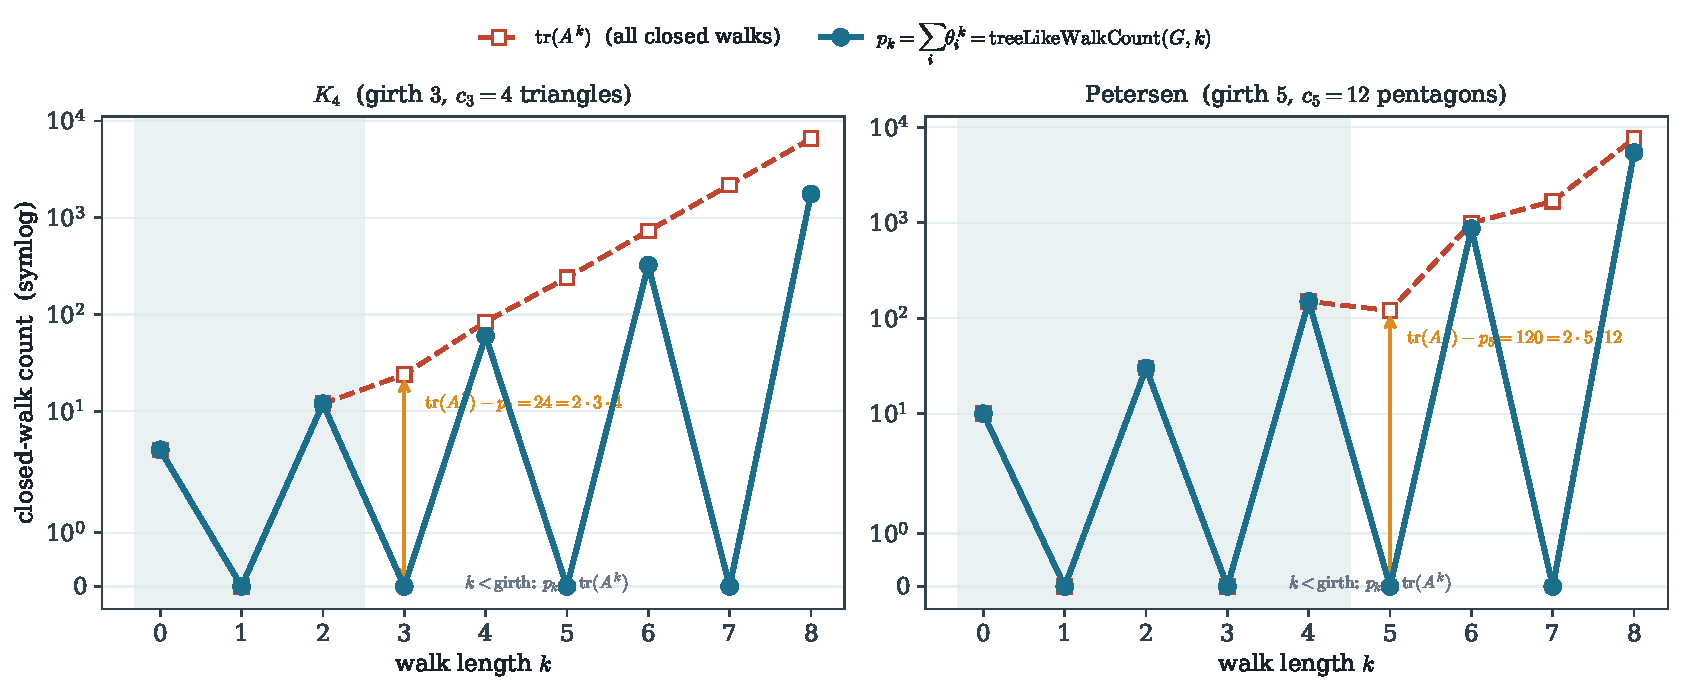
\includegraphics[width=0.98\textwidth]{figures/mt_fig1_traceformula.pdf}
  \caption{El teorema del momento como lado del \'arbol de la f\'ormula de la traza. Para $K_4$ (cuello
  $3$) y el grafo de Petersen (cuello $5$), las sumas de potencias $p_k=\sum_i\theta_i^{\,k}$ (verde
  azulado), que el Teorema~\ref{thm:moment} certifica iguales al conteo tipo \'arbol
  $\mathrm{treeLikeWalkCount}(G,k)=\sum_v[A(T(G,v))^k]_{\mathrm{ra\acute{\imath}z}}$, contra $\tr(A^k)$
  (rojo), el n\'umero de todos los caminos cerrados. Ambos coinciden por debajo del cuello (sombreado);
  el primer hueco, $\tr(A^g)-p_g=2g\,c_g$, cuenta los ciclos m\'as cortos ($g$ bases $\times\,2$
  orientaciones $\times\,c_g$ ciclos). Las sumas de potencias impares se anulan porque el polinomio de
  emparejamientos es par. El lado de los ciclos es el compa\~nero \emph{Bass} de esta serie; el lado
  del \'arbol es este art\'iculo.}
  \label{fig:traceformula}
\end{figure}

\begin{table}[t]
\centering\small
\caption{Las sumas de potencias $p_k=\sum_i\theta_i^{\,k}$, calculadas desde las ra\'ices de $\mu(G)$
en aritm\'etica exacta de $\overline{\mathbb{Q}}$, igualan el conteo del \'arbol de caminos
$\mathrm{treeLikeWalkCount}(G,k)$ de la Parte~III para todo $G$ y $k$ (el contenido del
Teorema~\ref{thm:moment}). Las $p_k$ impares se anulan. La \'ultima columna es el primer hueco de la
f\'ormula de la traza $\tr(A^{g})-p_{g}$ en $k=\mathrm{cuello}\;g$, que coincide con la ley de ciclos
m\'as cortos $2g\,c_g$.}
\label{tab:verify}
\rowcolors{2}{ggband!30}{white}
\begin{tabular}{@{}lccccccc@{}}
\toprule
\rowcolor{ggteal}
{\color{white}\textbf{$G$}} & {\color{white}$n$} & {\color{white}cuello} &
{\color{white}$p_0$} & {\color{white}$p_2$} & {\color{white}$p_4$} & {\color{white}$p_6$} &
{\color{white}$\tr(A^{g})-p_{g}=2g\,c_g$}\\
\midrule
$K_4$        & $4$  & $3$ & $4$  & $12$ & $60$  & $324$  & $24=2\cdot3\cdot4$\\
$C_5$        & $5$  & $5$ & $5$  & $10$ & $30$  & $100$  & $10=2\cdot5\cdot1$\\
$K_{3,3}$    & $6$  & $4$ & $6$  & $18$ & $90$  & $522$  & $72=2\cdot4\cdot9$\\
Petersen     & $10$ & $5$ & $10$ & $30$ & $150$ & $870$  & $120=2\cdot5\cdot12$\\
\bottomrule
\end{tabular}
\end{table}

% ---------------------------------------------------------------
\section{La frontera, ahora cerrada---y la ruta que la entrega anterior no predijo}
\label{sec:boundary}

\emph{La Parte~III map\'o esta conclusi\'on como ``la identidad del resolvente de una sola entrada y el
paso de Newton univariado''. El paso del resolvente est\'a aqu\'i, como se previ\'o. El paso de Newton
no---y su ausencia es lo \'unico matem\'aticamente interesante de la demostraci\'on.}

La secci\'on de frontera de la Parte~III esboz\'o una cadena de cinco eslabones hacia el teorema del
momento: la identidad del resolvente, el lema del menor principal, el puente del bosque, la identidad
de divisibilidad, la ley de borrado de v\'ertices, y luego una \emph{identidad de Newton univariada}
que igualaba la derivada logar\'itmica $\mu'/\mu$ con $\sum_k p_kX^k$. Cuatro de esos eslabones son
exactamente lo que usan las Secciones~\ref{sec:trace}--\ref{sec:weld}. El quinto no. No hay recursi\'on
de Newton en la formalizaci\'on, y no se a\~nadi\'o ning\'un lema de Newton de ra\'ices univariadas al
\'area de preparaci\'on de Mathlib.

Lo que lo reemplaz\'o es la cancelaci\'on de la Secci\'on~\ref{sec:match}: la generatriz
$\sum_\theta(1-\theta X)^{-1}$ multiplicada por $\prod_\theta(1-\theta X)$ se telescopa, al cancelarse
un solo factor, en la suma ``dejando uno fuera''
$\sum_\theta\prod_{\varphi\neq\theta}(1-\varphi X)$, que la regla del producto y una reflexi\'on
identifican con $\overline{X\mu'}$. Las identidades de Newton relacionan sumas de potencias con
funciones sim\'etricas elementales por una recursi\'on; aqu\'i el mismo contenido aparece como una sola
cancelaci\'on de multiconjuntos, con la derivada aportada por la regla del producto en lugar de por una
recursi\'on sobre $p_k$. La lectura por derivada logar\'itmica $\sum_kp_kX^k=n-X\,q'/q$ (con
$q=\rev(\mu)$) sigue siendo cierta---fue el anclaje num\'erico que de-arriesg\'o el paso---pero la
demostraci\'on formal nunca forma $q'/q$; trabaja con denominadores despejados en todo momento, por lo
que no necesita ni inverso ni recursi\'on. Es la clase de peque\~na sorpresa que una formalizaci\'on
saca a la luz: la ruta que en papel parece can\'onica (Newton) no es la m\'as barata ante la m\'aquina.

El lema del menor principal que la Parte~III se\~nal\'o como ``el \'unico lema de \'algebra lineal
genuinamente nuevo'' est\'a presente (\lean{adjugate\_diag\_eq\_det\_submatrix\_ne}), y tambi\'en su
hermano de determinante para una fila aislada (\lean{det\_eq\_det\_submatrix\_ne\_of\_row\_eq\_single});
ambos son libres de grafos y se guardan en forma can\'onica. El lema de reflexi\'on de una suma
(\lean{sum\_reverse\_eq\_reflect\_sum}) y el invertido de un producto descompuesto
(\lean{reverse\_prod\_X\_sub\_C}) son igualmente generales. Junto con el lado de los ciclos en el
compa\~nero \emph{Bass}~\cite{Bass}, la f\'ormula de la traza finita de emparejamientos/Ihara tiene ya
sus dos extremos---$\tr(A^k)$ contando todos los caminos cerrados y $p_k$ contando los tipo
\'arbol---en terreno certificado, en una sola biblioteca; por debajo del cuello sus coeficientes
coinciden como teoremas, y el primer hueco es un conteo de ciclos m\'as cortos, a la espera de ser
le\'ido.

% ---------------------------------------------------------------
\section{Implicaciones y metodolog\'ia}
\label{sec:methodology}

La formalizaci\'on y el manuscrito se desarrollaron con asistencia de IA (Claude, Anthropic); el autor
fij\'o los objetivos de investigaci\'on, juzg\'o la matem\'atica, y es responsable de todas las
afirmaciones. Todo teorema nombrado aqu\'i compila \lean{sorry}-libre contra la revisi\'on fijada de
Mathlib~\cite{Mathlib} y depende solo de los tres axiomas est\'andar, re-verificables con
\lean{\#print axioms}.

\paragraph{Un verde falso, y la lecci\'on guardada.} Una identidad
(\lean{godsil\_resolvent\_charpoly\_form}) estuvo, por un tiempo, silenciosamente rota: un
\lean{lake build} incremental reprodujo un objeto compilado obsoleto y report\'o \'exito mientras la
fuente ya no compilaba. La lecci\'on merece guardarse---que una compilaci\'on por objetivo pase no es
prueba de que un teorema compile; solo lo es una elaboraci\'on limpia del propio fichero---y cada
identidad de este art\'iculo se re-verific\'o elaborando su m\'odulo desde la fuente.

\paragraph{D\'onde se aplica, y c\'omo.} El teorema del momento es el puente entre dos maneras de leer
un grafo: como objeto combinatorio cuyos caminos se cuentan, y como portador de un espectro---que no
es de adyacencia del grafo---cuyos momentos se acotan. Es precisamente la identidad invocada, casi siempre t\'acitamente, all\'i
donde uno de ellos se estima a trav\'es del otro. En concreto:
\begin{itemize}
\item \emph{Cotas de autovalores por el m\'etodo de los momentos.} La mayor ra\'iz de emparejamiento
cumple $\theta_{\max}=\lim_k p_{2k}^{1/2k}$, y el teorema del momento convierte cada $p_{2k}$ en un
\emph{conteo de caminos} sobre el \'arbol de caminos---una cantidad combinatoria expl\'icitamente acotada,
dominada por los caminos en el cubrimiento universal $(\Delta-1)$-ario infinito, cuya densidad
espectral es la ley de Kesten--McKay~\cite{McKay,AngelFriedmanHoory}. Esta es la ruta a la cota de
Godsil $\theta_{\max}\le2\sqrt{\Delta-1}$, el an\'alogo en emparejamientos de la estimaci\'on del radio
espectral, y la $p_k$ certificada es su materia prima.
\item \emph{Umbrales de expansores y Ramanujan.} El borde de banda $2\sqrt{\Delta-1}$ que separa el
autovalor trivial de un grafo $\Delta$-regular del resto es el mismo n\'umero; un grafo de Ramanujan
es aquel cuyo espectro no trivial se mantiene dentro de \'el~\cite{MSS}. El teorema del momento liga la
versi\'on en ra\'ices de emparejamiento de ese umbral a un conteo tipo \'arbol, la forma en que la
comparaci\'on con el cubrimiento universal es m\'as limpia.
\item \emph{Mec\'anica estad\'istica.} $\mu(G,x)$ es la funci\'on de partici\'on mon\'omero--d\'imero;
sus ra\'ices son los ceros que controlan la ausencia de transici\'on de fase
(Heilmann--Lieb~\cite{HeilmannLieb}), y sus sumas de potencias $p_k$ son los momentos tipo cumulante
que produce una expansi\'on de alta temperatura. El teorema lee esos momentos de los caminos tipo
\'arbol del grafo.
\item \emph{Redes v\'ia el operador no-retrocedente.} El lado de los ciclos de la f\'ormula de la
traza, $\tr(A^k)$ y su refinamiento no-retrocedente $\tr(B^k)$, gobierna umbrales de percolaci\'on y
detecci\'on de comunidades en redes~\cite{Hashimoto,IharaBass}; el teorema del momento aporta el lado
del \'arbol contra el que esos conteos de ciclos se miden, y el primer hueco,
$\tr(A^g)-p_g=2g\,c_g$, es un conteo certificado de ciclos m\'as cortos.
\end{itemize}
Este art\'iculo no a\~nade ninguna cota ni ning\'un algoritmo a ninguno de ellos. Pone el \emph{puente
mismo}---la identidad exacta que cada uno cruza---en terreno certificado, en la misma biblioteca donde
el \'arbol de caminos ya porta un espectro real (Parte~II) y cuenta caminos tipo \'arbol (Parte~III).
El mismo bosque hace ahora un tercer trabajo: \emph{iguala} el conteo al espectro. Un cimiento, y el
cierre de un arco de cuatro partes.

\paragraph{El andamiaje formalizado.} La Tabla~\ref{tab:results} lista los resultados portantes, sus
nombres en Lean, y d\'onde se demuestra cada uno; los lemas generales y libres de grafos (marcados
$\ast$) se guardan en forma can\'onica para su env\'io a Mathlib.

\begin{table}[t]
\centering\small
\caption{Los resultados formalizados portantes. Todos son \lean{sorry}-libres contra la revisi\'on
fijada de Mathlib; $\ast$ marca los lemas generales y libres de grafos ausentes de Mathlib, guardados
para su env\'io aguas arriba.}
\label{tab:results}
\rowcolors{2}{ggband!30}{white}
\begin{tabular}{@{}llc@{}}
\toprule
\rowcolor{ggteal}
{\color{white}\textbf{Nombre en Lean}} & {\color{white}\textbf{Enunciado}} & {\color{white}\textbf{\S}}\\
\midrule
$\ast$\,\lean{det\_eq\_det\_submatrix\_ne\_of\_row\_eq\_single} & fila $i=e_i\Rightarrow\det M=\det(M\!\restriction_{\neq i})$ & \ref{sec:trace}\\
\lean{coe\_charpolyRev\_adjMatrix\_deleteIncidenceSet} & $\overline{\charpolyRev A(G_{\widehat r})}=\overline{\charpolyRev(A(G)\!\restriction_{\neq r})}$ & \ref{sec:trace}\\
\lean{resolventGenfun\_diag\_mul\_coe\_charpolyRev} & $\bigl(\sum_k[M^k]_{ii}X^k\bigr)\overline{\charpolyRev M}=\overline{\charpolyRev(M\!\restriction_{\neq i})}$ & \ref{sec:trace}\\
\lean{resolventGenfun\_pathTree\_mul\_reverse\_matchingPoly} & por v\'ertice: $\bigl(\sum_k[A(T)^k]_{\rm ra\acute{\imath}z}X^k\bigr)\overline{\mu(G)}=\overline{\mu(G-v)}$ & \ref{sec:trace}\\
$\ast$\,\lean{sum\_reverse\_eq\_reflect\_sum} & $\sum_i\rev(p_i)=\reflect_N(\sum_i p_i)$ si $\deg p_i=N$ & \ref{sec:trace}\\
\lean{mk\_treeLikeWalkCount\_mul\_reverse\_eq} & lado traza: $W(G)\,\overline{\mu(G)}=\overline{X\mu'(G)}$ & \ref{sec:trace}\\
\lean{geomSeries\_sum\_mul\_prod} & $\bigl(\sum_\theta\frac{1}{1-\theta X}\bigr)\prod_\theta(1-\theta X)=\sum_\theta\prod_{\varphi\neq\theta}(1-\varphi X)$ & \ref{sec:match}\\
$\ast$\,\lean{reverse\_prod\_X\_sub\_C} & $\rev\!\prod_\theta(X-\theta)=\prod_\theta(1-\theta X)$ & \ref{sec:match}\\
\lean{reflect\_X\_mul\_derivative\_eq\_sum\_prod} & $\sum_\theta\prod_{\varphi\neq\theta}(1-\varphi X)=\reflect_n(X\mu')$ & \ref{sec:match}\\
\lean{mk\_matchingPowerSum\_mul\_reverse\_eq} & lado empar.: $M(G)\,\overline{\mu_\C}=\overline{X\mu_\C'}$ & \ref{sec:match}\\
\lean{matchingPowerSum\_eq\_treeLikeWalkCount} & \textbf{teorema del momento:} $p_k(G)=\mathrm{treeLikeWalkCount}(G,k)$ & \ref{sec:weld}\\
\bottomrule
\end{tabular}
\end{table}

% ---------------------------------------------------------------
\section{Preguntas que quedan abiertas}
\label{sec:questions}

Una formalizaci\'on es tambi\'en una lista de las pr\'oximas preguntas, afiladas hasta que una m\'aquina
podr\'ia plante\'arselas.

\begin{itemize}
\item La demostraci\'on rodea la identidad de Newton. \,?`Es la cancelaci\'on de serie geom\'etrica
\emph{equivalente} a la recursi\'on de Newton univariada como lema de Mathlib---es decir, da una de
ellas una prueba corta de la otra---o son formas normales genuinamente distintas del mismo contenido,
una recursiva y otra cerrada?
\item Ambos lados fueron forzados a igualar $\overline{X\mu'}$. \,?`Puede refactorizarse la
demostraci\'on para que las dos generatrices se identifiquen \emph{antes} de la contabilidad de
reflexi\'on, puramente como cocientes de polinomios invertidos, dejando $\reflect_n$ fuera de la
cancelaci\'on?
\item Por debajo del cuello el teorema del momento da $p_k=\tr(A^k)$, y el primer hueco en
$k=\mathrm{girth}$ cuenta ciclos m\'as cortos. Ahora que ambos lados son objetos formales, \,?`puede
evaluarse el hueco $\tr(A^k)-p_k$ en $k=\mathrm{girth}$ dentro de la biblioteca, dando la correcci\'on
de conteo de ciclos $2\,\mathrm{girth}\cdot c_g$ como teorema?
\item La contabilidad de polinomios invertidos ($\rev$, $\reflect_N$, la unidad $\overline{\mu}$)
reaparece en los lados de emparejamientos e Ihara/Bass. \,?`Hay un solo c\'alculo de \emph{generatrices
invertidas} que subsuma ambos, de modo que la f\'ormula de la traza completa
$\tr(A^k)=p_k+(\text{t\'erminos de ciclo})$ sea una identidad en vez de dos mitades soldadas?
\item Los lemas del menor principal y de la reflexi\'on son generales. Llevados aguas arriba,
\,?`acortar\'ian desarrollos existentes de Mathlib---resultantes, matrices compa\~neras, la API actual
de \lean{charpolyRev}---o solo son \'utiles en compa\~n\'ia de un \'arbol de caminos?
\end{itemize}

Y una para guardar. \emph{El polinomio de emparejamientos no es el polinomio caracter\'istico de la
matriz de adyacencia del propio grafo y, sin embargo, las sumas de potencias de sus ra\'ices cuentan
caminos exactamente como lo har\'ian las de un espectro; el teorema dice d\'onde viven esos momentos---pero el espectro que
describen, \,?`es un artefacto contable del \'arbol de caminos, o, para todo uso que consuma sus
momentos, tan real como el de cualquier matriz?}

% ---------------------------------------------------------------
\begin{thebibliography}{99}

% --- el polinomio de emparejamientos y sus raices reales ---
\bibitem{HeilmannLieb} O.~J. Heilmann and E.~H. Lieb, \emph{Theory of monomer--dimer systems},
Comm.\ Math.\ Phys.\ \textbf{25} (1972), 190--232.
\bibitem{Farrell1979} E.~J. Farrell, \emph{An introduction to matching polynomials}, J.~Combin.\
Theory Ser.~B \textbf{27} (1979), 75--86.
\bibitem{LovaszPlummer} L.~Lov\'asz and M.~D. Plummer, \emph{Matching Theory}, North-Holland Math.\
Stud.\ \textbf{121}, Amsterdam, 1986.

% --- el arbol de caminos de Godsil: emparejamientos, caminos, y el teorema del momento ---
\bibitem{Godsil1981a} C.~D. Godsil, \emph{Matchings and walks in graphs}, J.~Graph Theory \textbf{5}
(1981), 285--297.
\bibitem{Godsil1981b} C.~D. Godsil and I.~Gutman, \emph{On the theory of the matching polynomial},
J.~Graph Theory \textbf{5} (1981), 137--144.
\bibitem{GodsilBook} C.~D. Godsil, \emph{Algebraic Combinatorics}, Chapman \& Hall, New York, 1993.

% --- las identidades de Newton, la ascendencia de funciones simetricas ---
\bibitem{Girard} A.~Girard, \emph{Invention nouvelle en l'alg\`ebre}, Amsterdam, 1629.
\bibitem{Macdonald} I.~G. Macdonald, \emph{Symmetric Functions and Hall Polynomials}, 2nd ed.,
Oxford Univ.\ Press, 1995.

% --- cubrimientos universales, espectros no-retrocedentes, el polinomio de emparejamientos ---
\bibitem{AngelFriedmanHoory} O.~Angel, J.~Friedman, and S.~Hoory, \emph{The non-backtracking spectrum
of the universal cover of a graph}, Trans.\ Amer.\ Math.\ Soc.\ \textbf{367} (2015), 4287--4318.
\bibitem{Spier2025} T.~J. Spier, \emph{Eigenvalues of universal covers and the matching polynomial},
preprint, 2025. \texttt{arXiv:2510.05041}.
\bibitem{McKay} B.~D. McKay, \emph{The expected eigenvalue distribution of a large regular graph},
Linear Algebra Appl.\ \textbf{40} (1981), 203--216.
\bibitem{GodsilMoments} C.~D. Godsil, \emph{Walk generating functions, Christoffel--Darboux
identities and the adjacency matrix of a graph}, Combin.\ Probab.\ Comput.\ \textbf{1} (1992),
13--25.

% --- la zeta de Ihara / el lado de los ciclos ---
\bibitem{Hashimoto} K.~Hashimoto, \emph{Zeta functions of finite graphs and representations of
$p$-adic groups}, in \emph{Automorphic Forms and Geometry of Arithmetic Varieties}, Adv.\ Stud.\
Pure Math.\ \textbf{15}, 1989, 211--280.
\bibitem{IharaBass} H.~Bass, \emph{The Ihara--Selberg zeta function of a tree lattice}, Internat.\
J.~Math.\ \textbf{3} (1992), 717--797.

% --- grafos de Ramanujan (el borde de banda $2\sqrt{\Delta-1}$) ---
\bibitem{MSS} A.~Marcus, D.~A. Spielman, and N.~Srivastava, \emph{Interlacing families~I: Bipartite
Ramanujan graphs of all degrees}, Ann.\ of Math.\ \textbf{182} (2015), 307--325.

% --- esta serie (formalizaciones Lean 4 / Mathlib) ---
\bibitem{PartI} C.~Mar\'in, \emph{Random Signs into Matchings: the Godsil--Gutman estimator and
real-rootedness in Lean~4} (Parte~I), 2026. Zenodo, DOI \texttt{10.5281/zenodo.20517350}.
\bibitem{PartII} C.~Mar\'in, \emph{Unfolding a Graph into a Tree: A Machine-Checked Proof of the
Heilmann--Lieb Theorem in Lean~4} (Parte~II), 2026. Zenodo, DOI \texttt{10.5281/zenodo.20561832}.
\bibitem{Bass} C.~Mar\'in, \emph{Folding Edges into Vertices: A Machine-Checked Proof of Bass's
Determinant Formula for the Ihara Zeta in Lean~4}, 2026. Zenodo, DOI
\texttt{10.5281/zenodo.20573120}.
\bibitem{PartIII} C.~Mar\'in, \emph{Walks that Forget the Cycles: A Machine-Checked Bijection between
Tree-Like Walks of a Graph and Walks on Godsil's Path Tree, in Lean~4} (Parte~III), 2026. Zenodo, DOI
\texttt{10.5281/zenodo.20600326}.

% --- el asistente de demostracion ---
\bibitem{Mathlib} The mathlib Community, \emph{The Lean mathematical library}, in \emph{Proc.\ 9th
ACM SIGPLAN Int.\ Conf.\ on Certified Programs and Proofs} (CPP~2020), 367--381.

\end{thebibliography}

\end{document}
